\section{Resultados}\label{sec:resultados}

En el siguiente apartado se muestran los resultados de ejecutar el código planteado para la creación de la respuesta, tanto de impulso como de frecuencia del pulso coseno alzado para distintos factores $roll-off$, además de la creación del diagrama de ojo junto con la aplicación del filtro AWGN.

Para realizar lo anterior mencionado, se utilizaron de manera general los siguientes parámetros.

\begin{equation}\label{eq:frecuencia coseno alzado}
    \begin{split} 
    &Frecuencia =  1000\\
    &Periodo\ de\ sincronizacion = \frac{1}{1000}  [Ts] \\
    &Frecuencia\ de\ muestreo\ de\ Nyquist = 10000\\
    &Periodo\ de\ muestreo = \frac{1}{10000} [tm] \\
    &Muestras\ para\ un\ periodo\ de\ sincronizacion = \frac{ts}{tm}\\
    &Factores\ roll-off = 0-0.25-0.75-1\\
    \end{split} 
\end{equation} 


\subsection{Actividad 1 }

En las siguientes imágenes, se muestra el resultado de aplicar distintos factor de $roll-off$ a la respuesta de impulso del coseno alzado y a la frecuencia del coseno alzado:


\subsubsection{Impulso roll-off 0} \phantom{text} %coloque esto porque las imagenes se agilan
\begin{figure}[H]
    \centering
    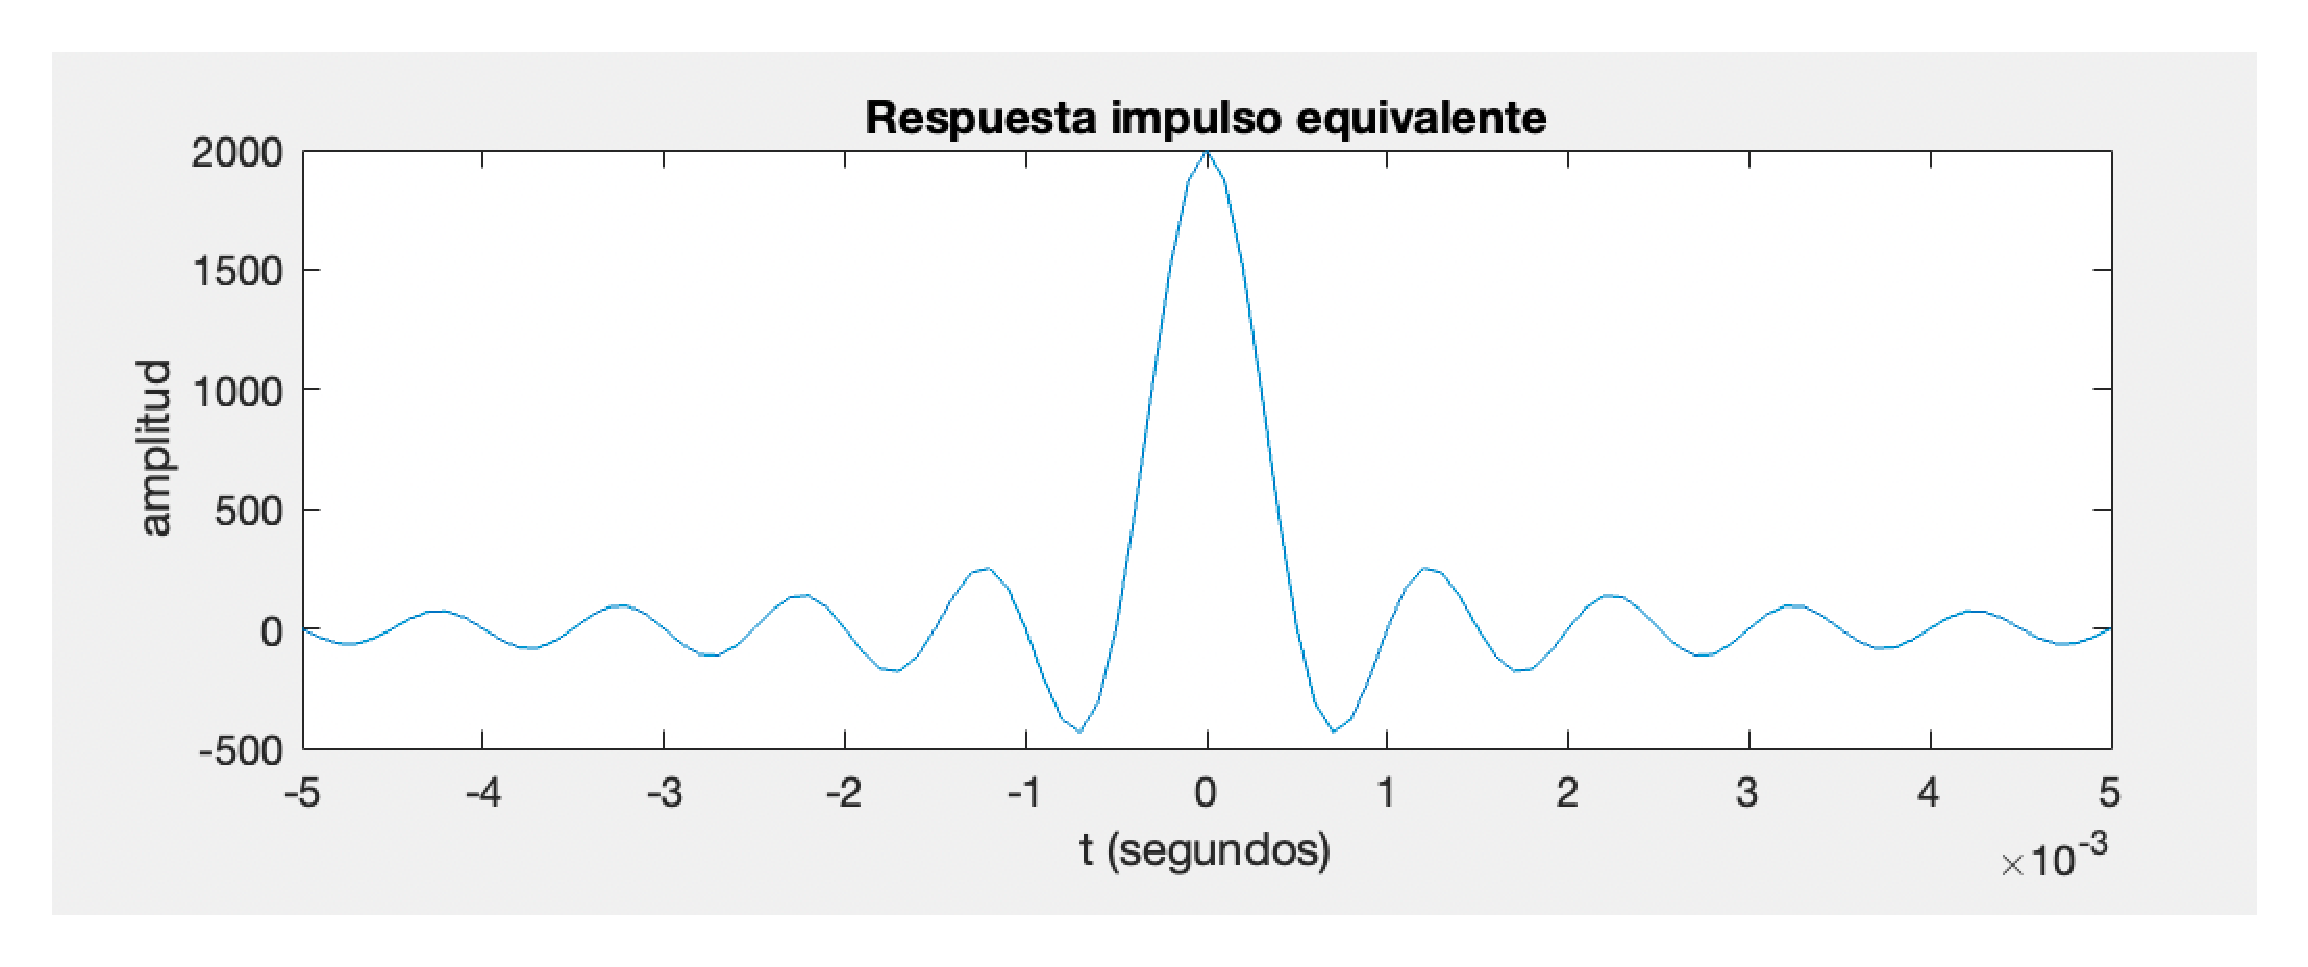
\includegraphics[scale=0.22]{Imagenes/act 2/frecuenciarollof0.pdf}
    \caption{Respuesta en impulso  con roll-off de 0}
    \label{fig:Respuesta en frecuencia  con roll-off de 0}
\end{figure}


\subsubsection{Frecuencia roll-off 0} \phantom{text}

\begin{figure}[H]
    \centering
    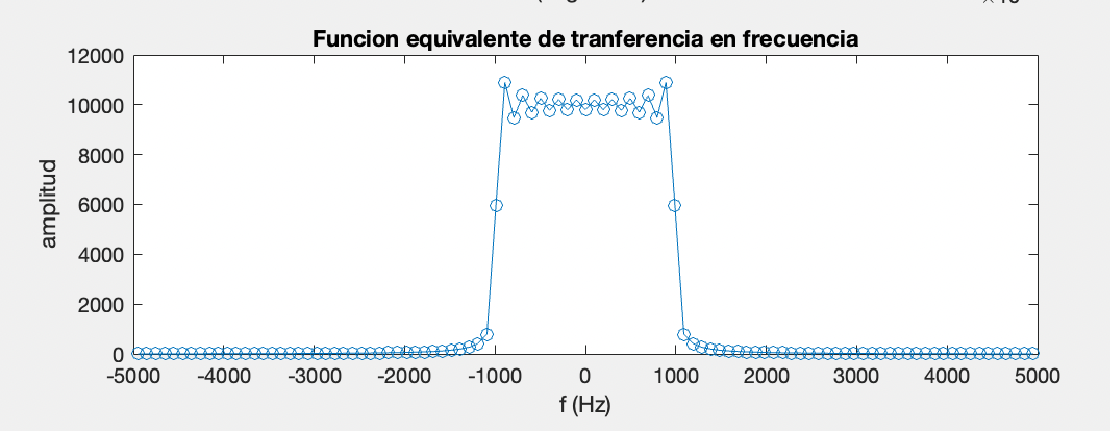
\includegraphics[scale=0.45]{Imagenes/act 2/impuslorollof0.pdf}
    \caption{Respuesta en impulso con roll-off de 0}
    \label{fig:Respuesta al impulso con roll-off de 0}
\end{figure}



\subsubsection{Impulso roll-off 0.25} \phantom{text}

\begin{figure}[H]
    \centering
    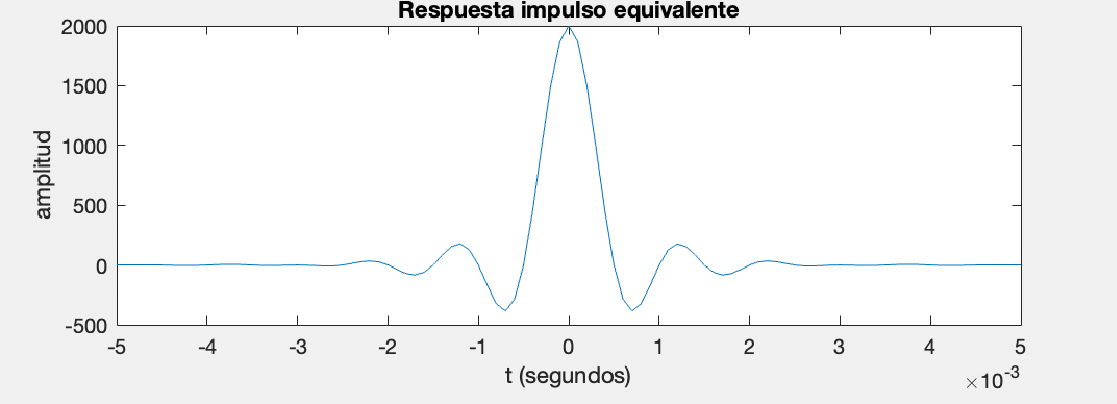
\includegraphics[scale=0.4]{Imagenes/act 2/rolloff0.25imp.pdf}
    \caption{Respuesta al impulso con roll-off de 0.25}
    \label{fig:Respuesta al impulso con roll-off de 0.25}
\end{figure}


\subsubsection{Frecuencia roll-off 0.25} \phantom{text}

\begin{figure}[H]
    \centering
    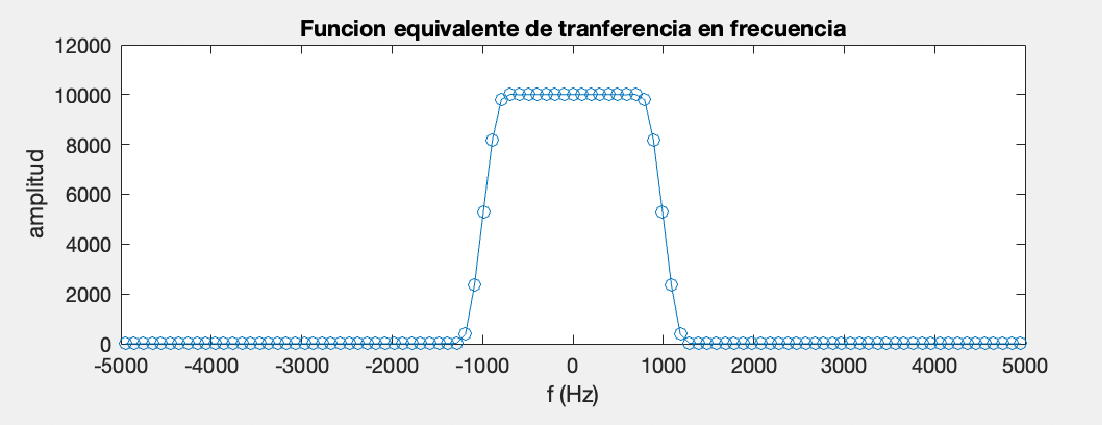
\includegraphics[scale=0.4]{Imagenes/act 2/rolloff0.25frec.pdf}
    \caption{Respuesta en  frecuencia  con roll-off de 0.25}
    \label{fig:Respuesta en  frecuencia  con roll-off de 0.25}
\end{figure}


\subsubsection{Impulso roll-off 0.75} \phantom{text}

\begin{figure}[H]
    \centering
    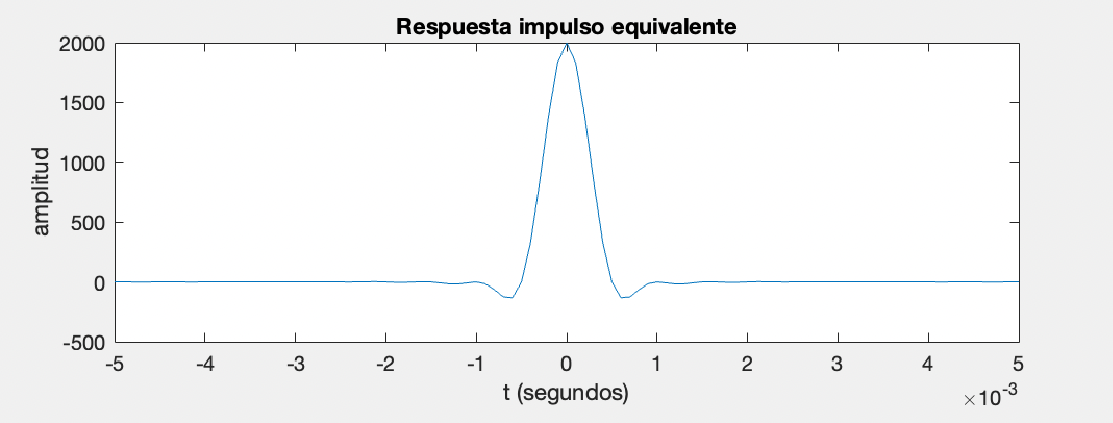
\includegraphics[scale=0.4]{Imagenes/act 2/rollof0.75imp.pdf}
    \caption{Respuesta al impulso con roll-off de 0.75}
    \label{fig:Respuesta al impulso con roll-off de 0.75}
\end{figure}


\subsubsection{Frecuencia roll-off 0.75} \phantom{text}

\begin{figure}[H]
    \centering
    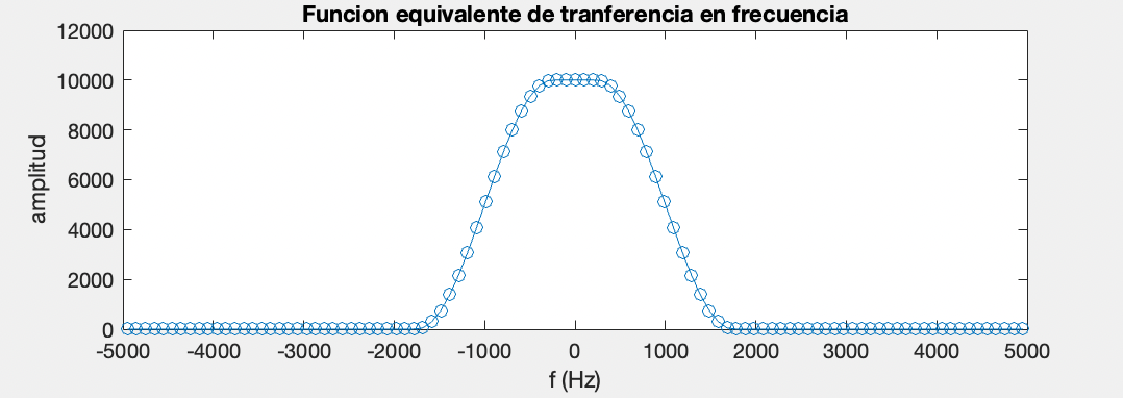
\includegraphics[scale=0.4]{Imagenes/act 2/rolloff0.75frec.pdf}
    \caption{Respuesta en  frecuencia  con roll-off de 0.75}
    \label{fig:Respuesta en  frecuencia  con roll-off de 0.75}
\end{figure}


\subsubsection{Impulso roll-off 1} \phantom{text}

\begin{figure}[H]
    \centering
    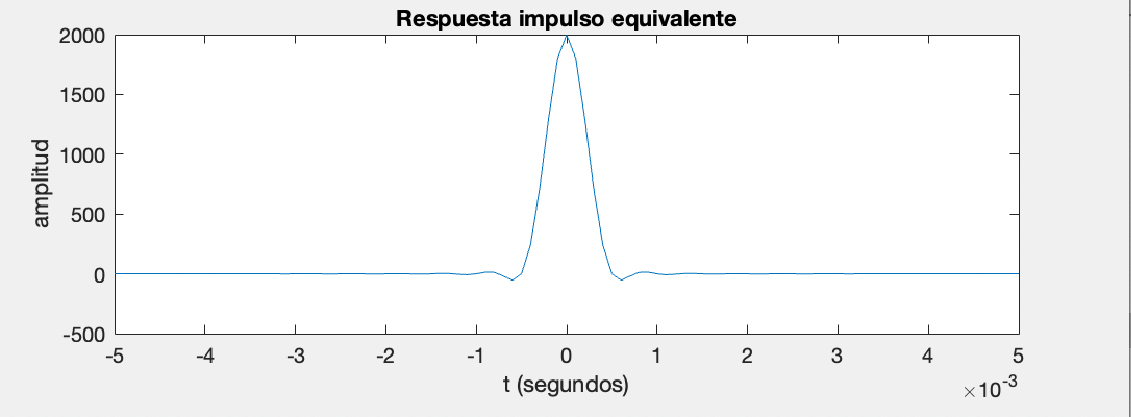
\includegraphics[scale=0.4]{Imagenes/act 2/rolloff1imp.pdf}
    \caption{Respuesta al impulso con roll-off de 1}
    \label{fig:Respuesta al impulso con roll-off de 1}
\end{figure}


\subsubsection{Frecuencia roll-off 1} \phantom{text}

\begin{figure}[H]
    \centering
    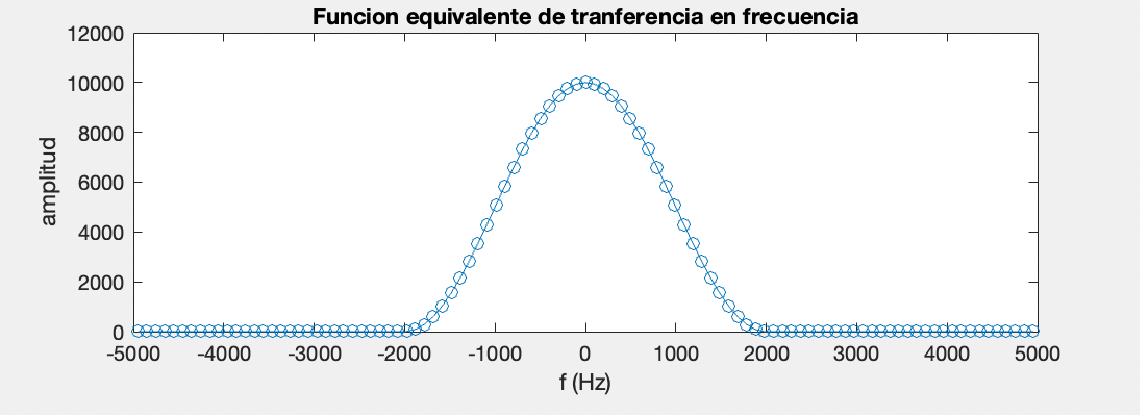
\includegraphics[scale=0.4]{Imagenes/act 2/rolloff1frec.pdf}
    \caption{Respuesta en  frecuencia  con roll-off de 1}
    \label{fig:Respuesta en  frecuencia  con roll-off de 1}
\end{figure}


\subsection{Actividad 2}


En el siguiente apartado se muestra los resultados al ejecutar el código planteado para la creación  del diagrama de ojo para el pulso de coseno alzado, por otra parte se vera las consecuencias de modificar las frecuencias de muestreo y el factor roll-off de este pulso.



\vspace*{-0.5cm}
\begin{figure}[H]
    \centering
    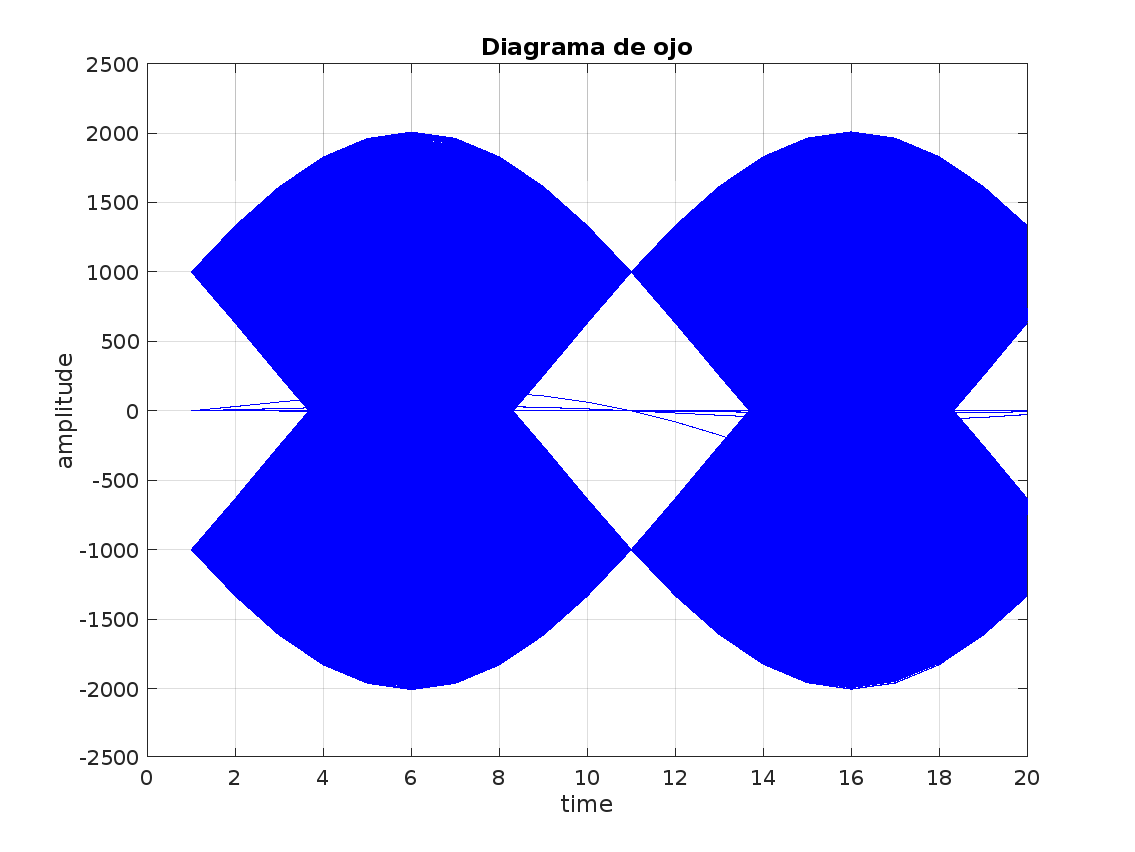
\includegraphics[scale=0.4]{Imagenes/DiagramaOjo/Figure_1rollOff022.pdf}
    \caption{Diagrama ojo a partir de roll-off 0.22}
    \label{fig:Diagrama ojo awgn}
\end{figure}

\vspace*{-1cm}
\begin{figure}[H]
    \centering
    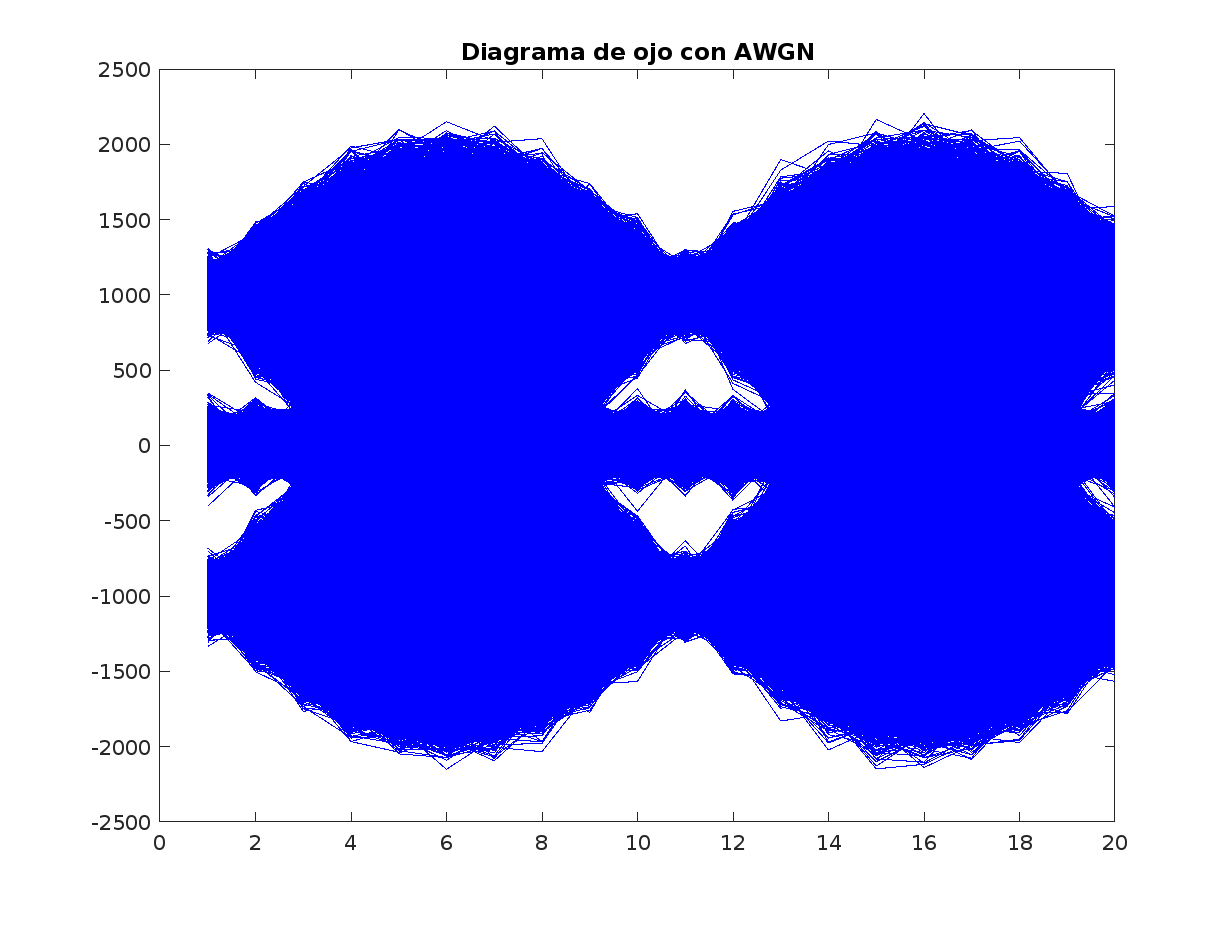
\includegraphics[scale=0.4]{Imagenes/DiagramaOjo/Figure_2roolOff022.pdf}
    \caption{Diagrama ojo AWGN a partir del roll-off 0.22}
    \label{fig:Diagrama ojo awgn}
\end{figure}

\vspace{-1cm}
\subsection{Cuestionario}


\begin{enumerate}
    \item \textbf{¿Que pasa si disminuye la frecuencia de muestreo?}
    \textbf{R:}
    Al disminuir la frecuencia de muestreo, se generó el siguiente diagrama de ojo.
    
    \begin{figure}[H]
    \centering
    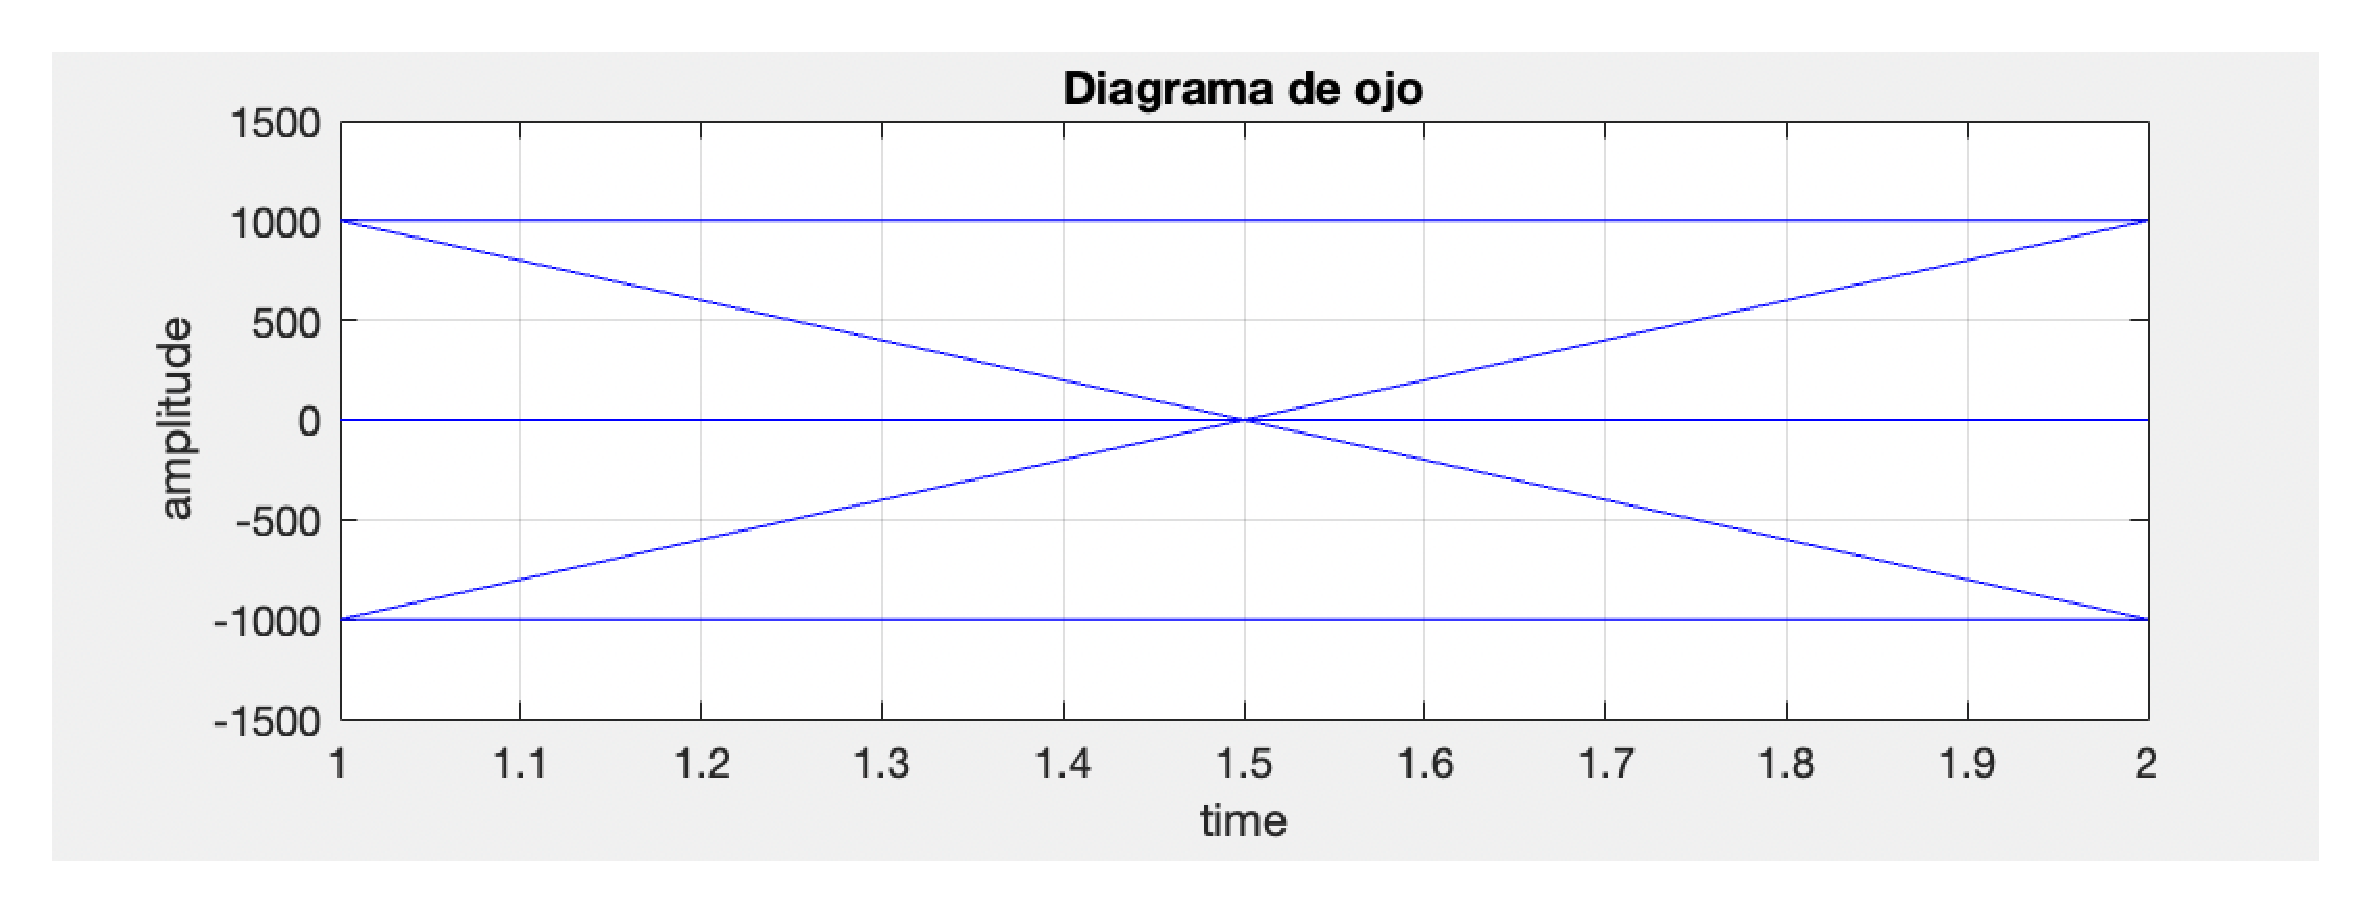
\includegraphics[scale=0.18]{Imagenes/DiagramaOjo/do.pdf}
    \caption{Diagrama ojo con frecuencia de muestreo equivalente a 1000}
    \label{fig:Diagrama ojo con frecuencia de muestreo baja}
\end{figure}

Donde se observa que si, al disminuir considerablemente la frecuencia de muestreo del pulso coseno alzado se estaría restringiendo considerablemente el ancho de banda de este mismo, esto ocurre siempre y cuando el cambio de frecuencia de muestreo sea considerable. En caso contrario de que la modificación sea menor, la restricción al ancho de banda no será significativa, sin embargo no influye en que genere una pérdida de muestras.

    \item \textbf{En forma general, ¿Qué sucede al incrementar el valor de $\alpha$?}\\
    \textbf{R:}    Al ir incrementando el factor roll-off, el diagrama de ojo generado por el pulso coseno alzado poseerá un mayor ancho de banda en comparación a pulsos de menor valor de factor roll-off, además el coseno alzado poseerá un ancho de banda superior al pulso cuadrado  (dependiendo del factor que se utilice), ya que por definición el factor roll-off($\alpha$) establece  el porcentaje de ancho de banda que supera  el pulso del coseno alzado con respecto al ancho de banda que ocupa el pulso rectangular.\cite{WinNT:filtro}
   
    
    Por otra parte al ir aumentando el roll-off, se va solucionando el problema de $"$ jitter$"$ que es la fluctuación del retardo de señales \cite{WinNT:jitter}, esto a mayor roll-off la fluctuación es casi nula permitiendo que la señal pase por 0 en el mismo instante relativo.
    


\end{enumerate}